% Rules for the HuroCup Weight Lifting Competition
% Jacky Baltes <jacky@cs.umanitoba.ca> 

\documentclass[12pt]{hurocup}
\begin{document}

\title{\HuroCup: Weight Lifting\\
  Laws of the Game 2007}


\author{Jacky Baltes\\
Autonomous Agents Laboratory\\
University of Manitoba\\
Winnipeg, Manitoba\\
Canada, R3T 2N2\\
Email: jacky@cs.umanitoba.ca\\
WWW: http://www.cs.umanitoba.ca/\~{ }jacky
}

\maketitle
\begin{abstract}
The following rules and regulations govern the Weight Lifting event in
\HuroCup, a robotic game and robotics benchmark problem for humanoid
robots.
%
\end{abstract}

\section*{Latest Version of the Rules for \HuroCup}
\label{sec:updates}

The latest official version of the rules of the game for \HuroCup\ is
always available from the FIRA \HuroCup\ website (http://www.fira.net).

\newpage

\section{Weight Lifting}
\label{sec:weight-lifting} 

The goal of the weight lifting competition is to encourage research in
actively balancing and carrying robots.

\section{Changes in the Laws of \HuroCup\ for 2007}

The year 2007 marks a big change in the history of \HuroCup\ as it will
be the inaugural competiton for the \HuroCup, which greatly increases
the status and scope of humanoid robotics competitions within the FIRA
framework.

\section{Laws of the Game: Weight Lifting}
\label{sec:weight-lifting-laws}

The following laws describe the specifics of the weight lifting
event. For general specifications relevant to all \HuroCup\ events
(e.g., robot dimensions, playing field and lighting, responsibility of
the referees) please refer to the general \HuroCup\ laws.

\law[WL]{The Field of Play}
\label{mr-field}

\begin{lawlist}[WL]
\item The weight lifting competition is played on a field with a
minimum dimension of 1.8m by 1.8m.

\item There are three lines marked on the playing field: (a) the start line,
 (b) the lift line, and (c) the final line. The distance between the
 start line and the lift line and the lift line and the finish line is
 30cm for small robots and 50cm for large robots.

\item Teams may place small coloured or infra red markers in the area
 behind the end zone to guide the robot as long as they do not
 interfere with other teams.

\begin{figure}
  \begin{center}
    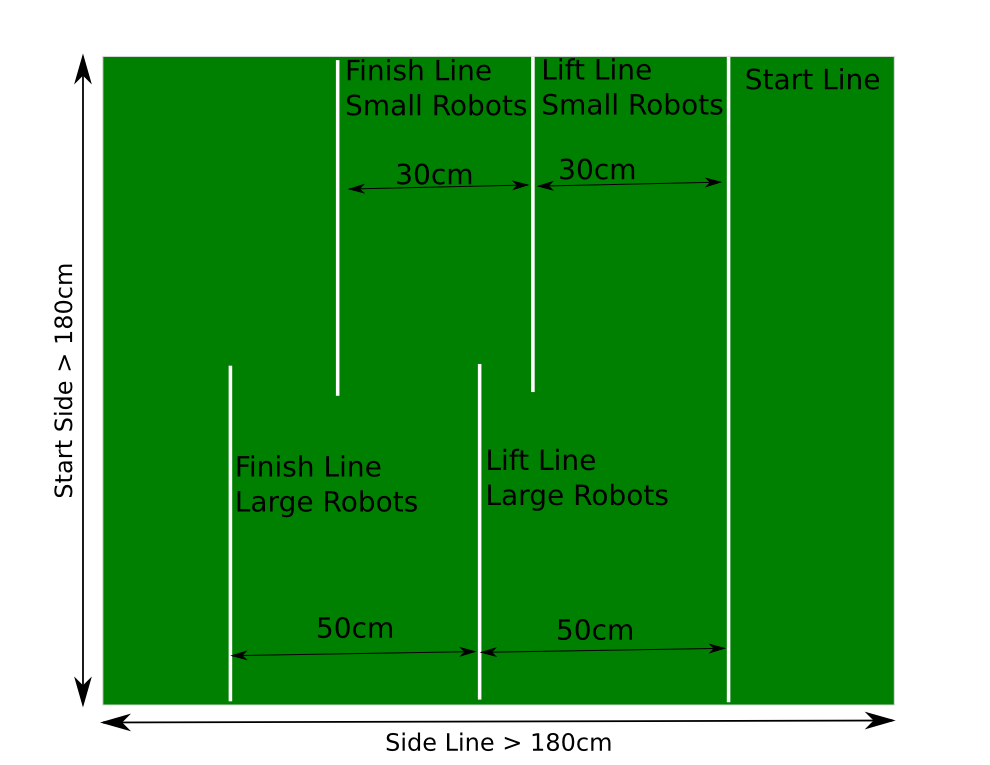
\includegraphics[width=0.70\linewidth]{Figures/weight-lifting}
  \end{center}
\end{figure}

\end{lawlist}

\law[WL]{The Lifting Bar and the Weights}

\begin{lawlist}[WL]

\item The lifting bar is a wodden, metal, or plastic bar with a width
 between 8 mm to 15mm. Two stops are used to mount the weights. The
distance between the inner stops is 30cm. The total length of the
lifting bar is between 40 - 50cm.

\item The ``weights'' used in the competition are standard 5 1/4 inch
 CDs or DVDs that must be lifted by the robot as seen in
 Fig.~\ref{fig:lifting-bar}.

\begin{figure}
\begin{center}
\begin{tabular}{cc}
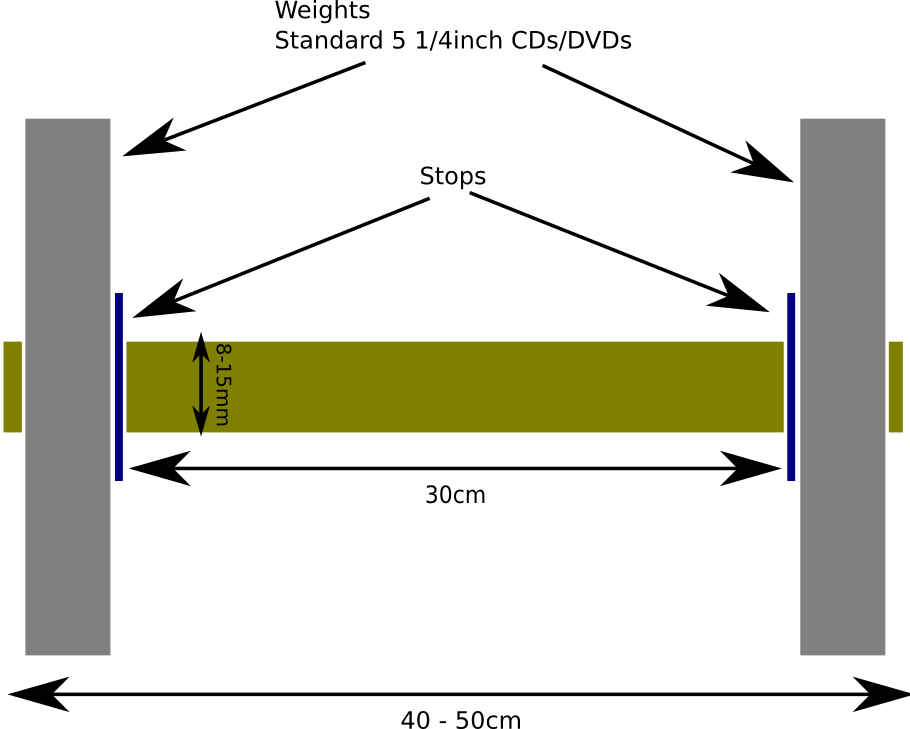
\includegraphics[width=0.4\linewidth]{Figures/lifting-bar-diagram} 
&
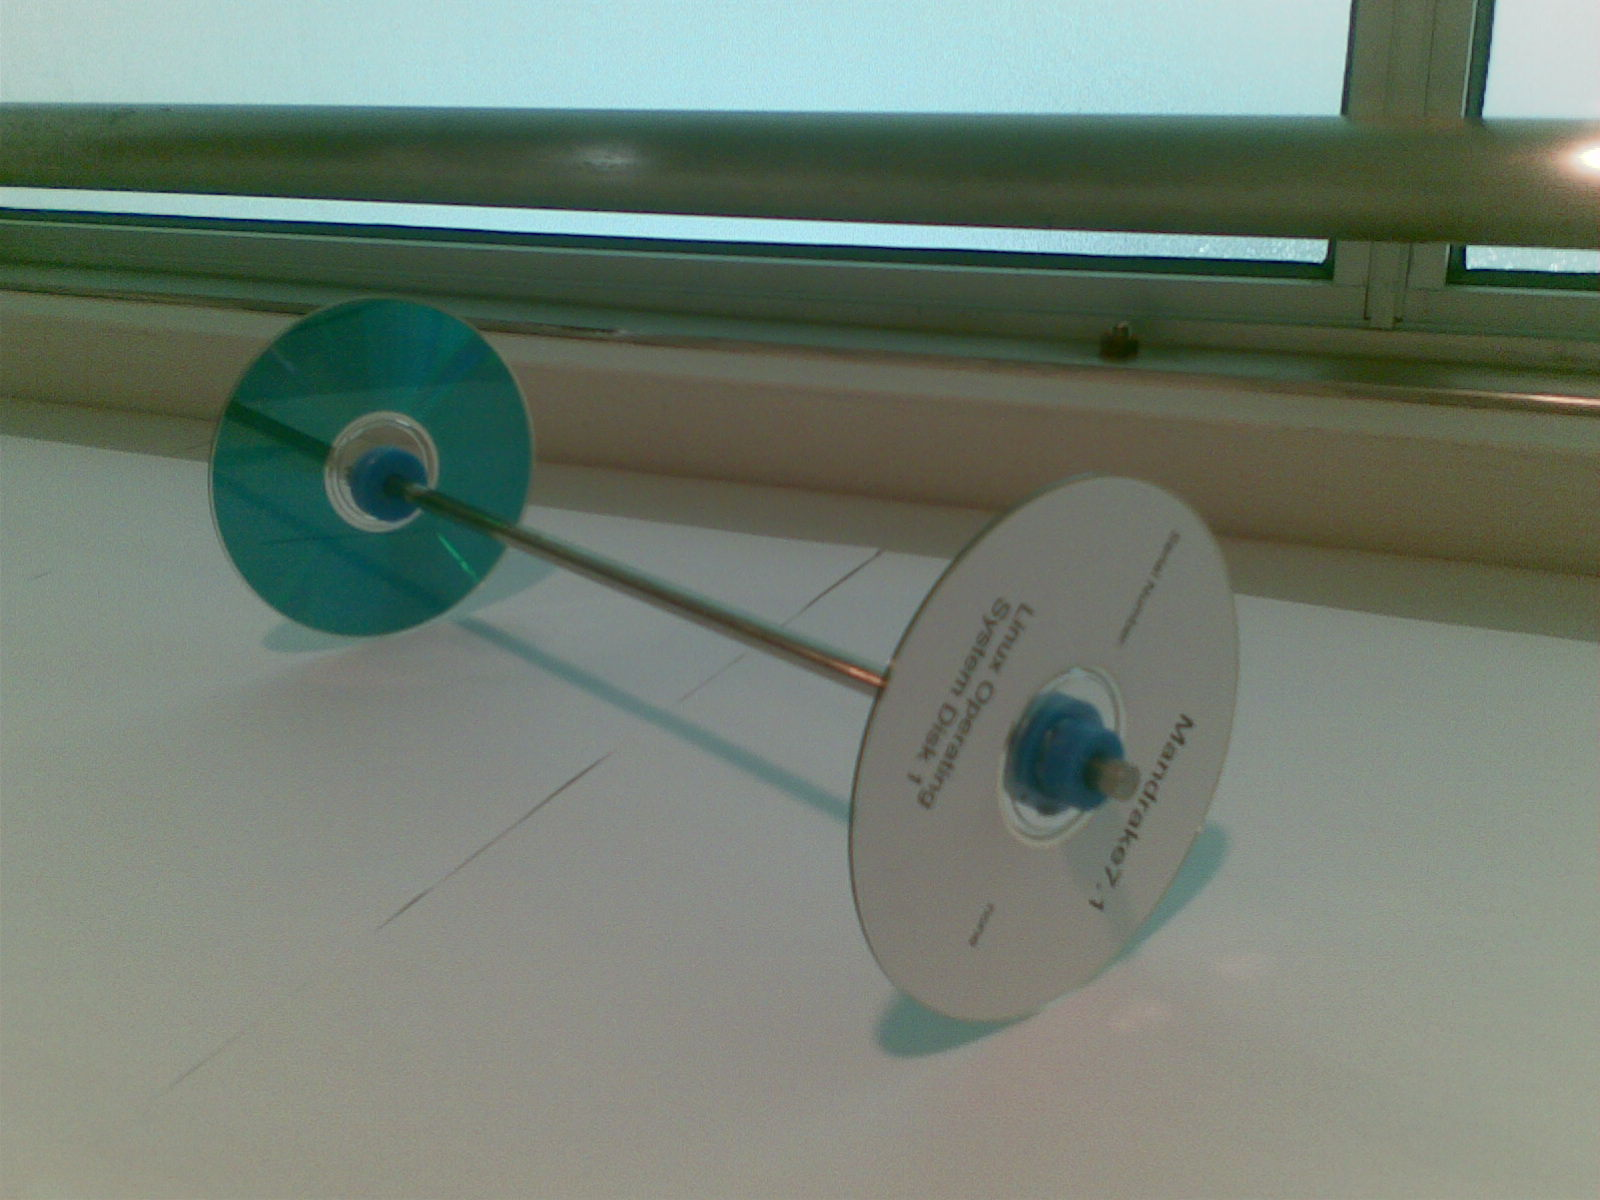
\includegraphics[width=0.4\linewidth]{Figures/lifting-bar1} 
\end{tabular}
\caption{Lifting Bar: A schematic and a picture of a possible lifting
bar.}
\label{fig:lifting-bar}
\end{center}
\end{figure}

\end{lawlist}

\law[WL]{Number of Robots}

\begin{lawlist}[WL]
\item A single robot competes in a match.
\end{lawlist}

\law[WL]{The Players}

Please refer to the general \HuroCup\ laws for a description of
the players.

\law[WL]{The Referee}

Please refer to the general \HuroCup\ laws for a description of
the referee.

\law[WL]{The Assistant Referee}

Please refer to the general \HuroCup\ laws for a description of
the assitant referee.

\law[WL]{Game Play}

\begin{lawlist}[WL]

\item A single robot is designated the lifter. All other robots
  must be outside of the playing field.

\item The only robot allowed to move during a run is the
  designated lifter.

\item The lifter will be placed behind the start line.

\item At the beginning of the try, the team will inform the
 referee how many CDs the team wants to attempt to lift and the
 referee will attach the desired weight to the lifting bar.

\item The referee will signal the start of the competition by blowing
  the whistle.

\item After the referee gives the start signal, the robot must cross
 the lifting line while carrying the weight below head height of the
 robot.

\item While touching the lifting line, the robot must lift the lifting
 bar above its head. The height difference between the low and heigh
 position must be at least 10cm.

\item While keeping the lifting bar above its head, the robot must
 continue to walk towards the finish line. A lift is considered
 successful if the robot crosses the finish line with the weight above
 its head.

\begin{figure}
\begin{center}
\begin{tabular}{cc}
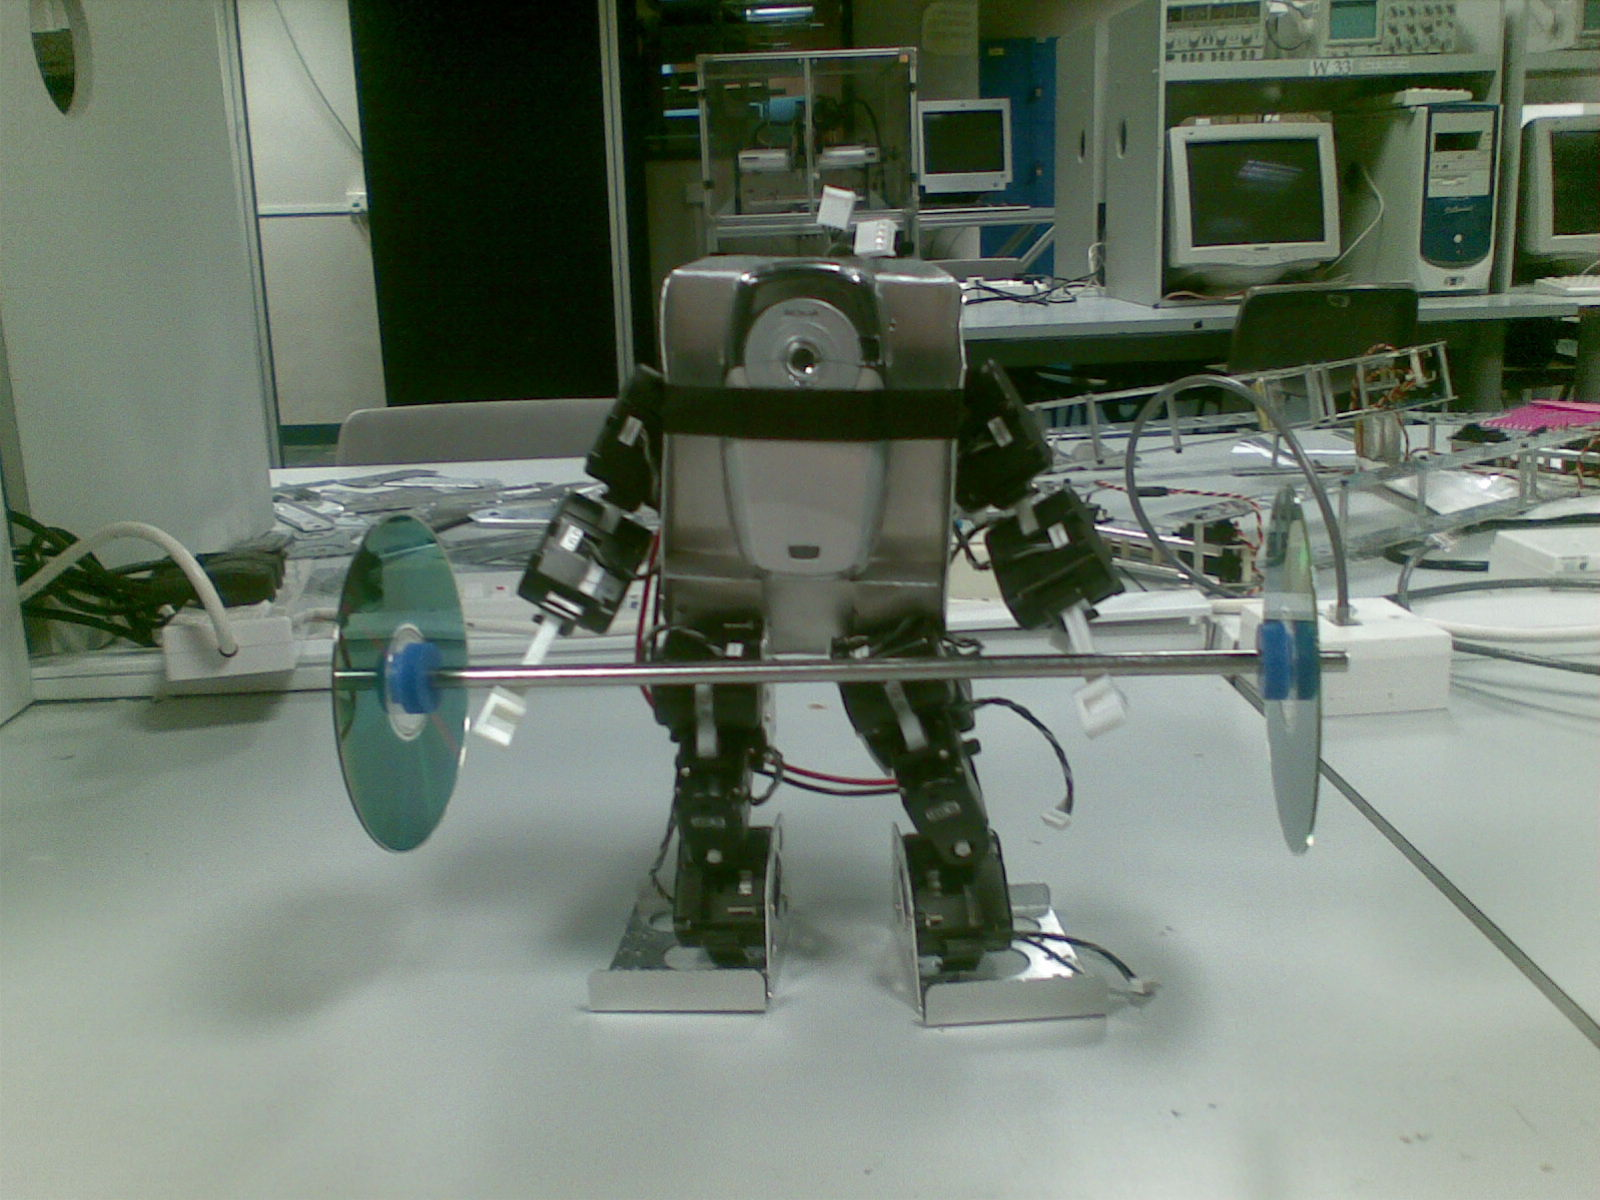
\includegraphics[width=0.4\linewidth]{Figures/weight-lifting1} 
&
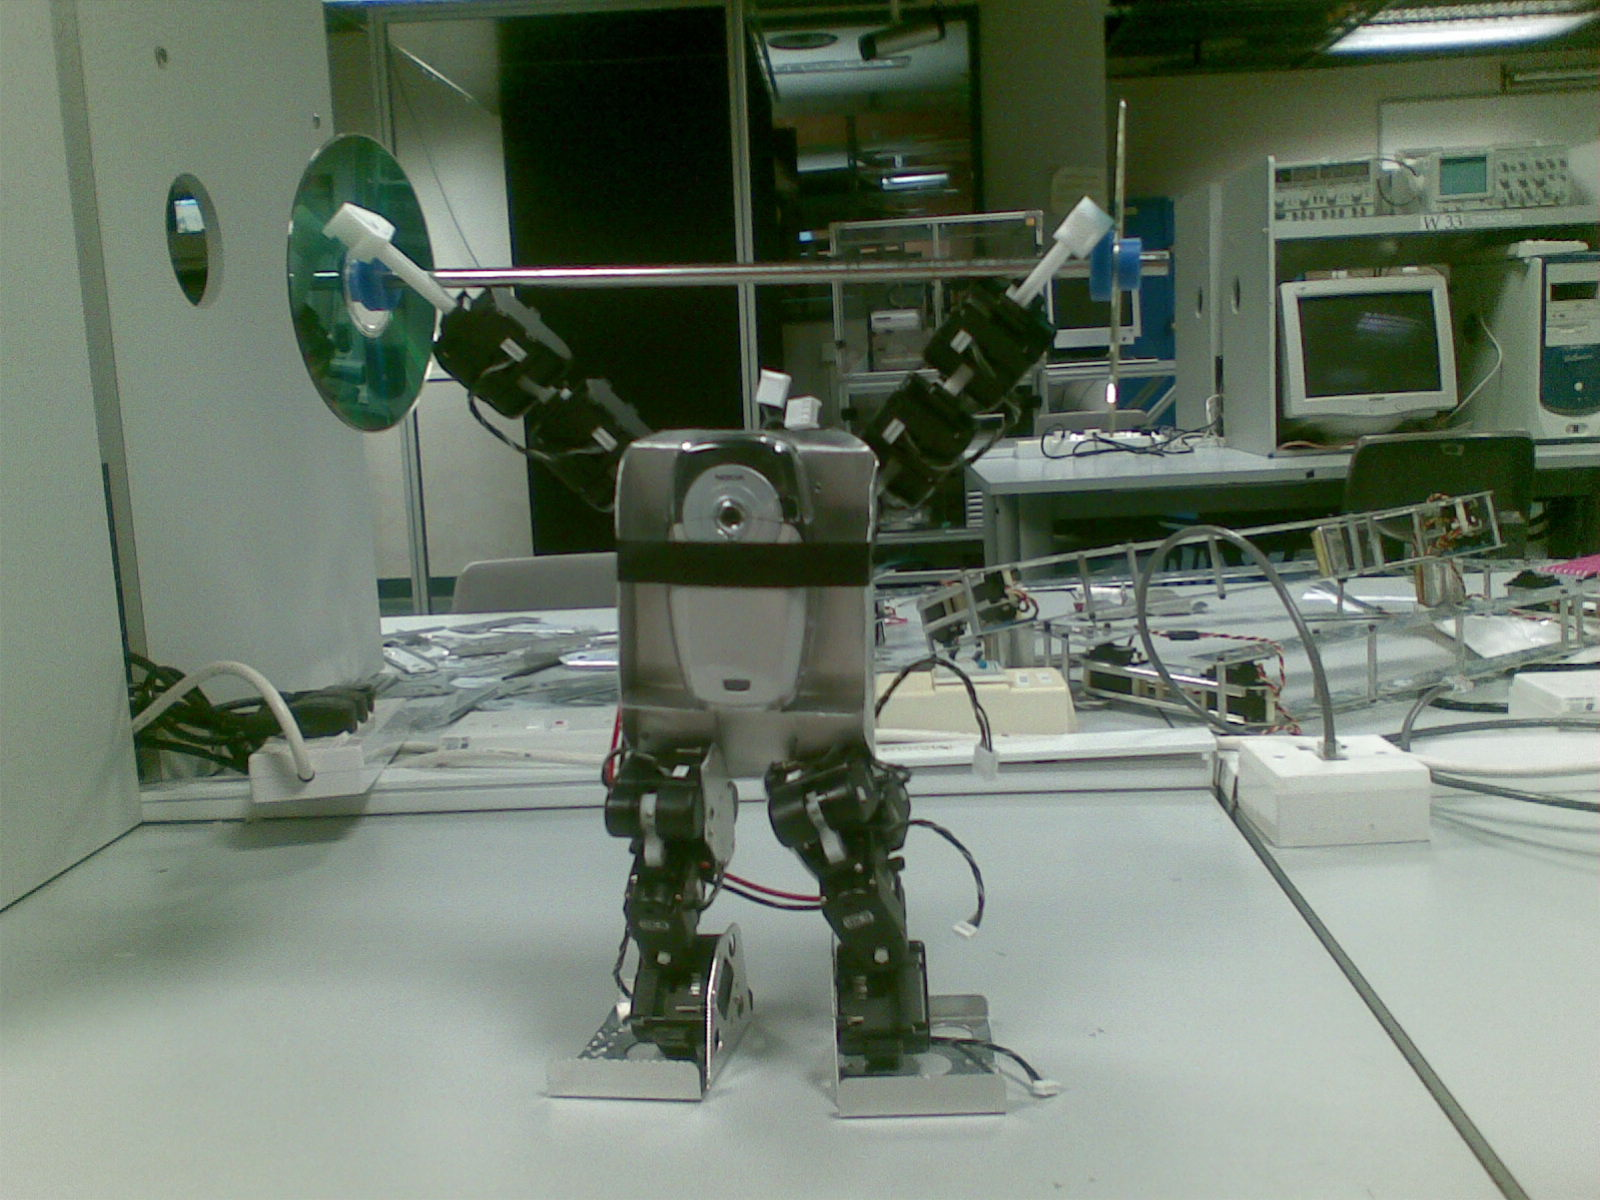
\includegraphics[width=0.4\linewidth]{Figures/weight-lifting2} 
\end{tabular}
\caption{A robot carrying the lifting bar below and above the head.}
\label{fig:weight-lifting}
\end{center}
\end{figure}

\item A robot is not allowed to leave the playing field.

\item Each robot may have at most one human handler associated with
  it.

\item \label{lc-handler5} The human handlers are not allowed to
  interfere in any way with other robots, the referee, or other human
  handlers.

\item \label{lc-handler6} A human handler may only enter the playing
 field or touch his/her robot with the permission of the referee.

\item The end of the competition is signaled by the referee by
  blowing the whistle a second time.
  The referee terminates the competition if
  \begin{itemize}
  \item the robot has successfully crossed the finish line,
  \item the robot was unable to complete the try within 2 minutes,
  \item the robot falls and is unable to get up on its own or is
    immobilized by a technical defect, 
  \item the robot leaves the playing field,
  \end{itemize}

\item A robot may continue in the competition as long as it has failed
 less than three tries. When the robot will be declared the lifter in
 the next round, then the team may choose a new weight for the next
 try. 

\item At the end of the try, another robot will be designated the
 lifter. 

\end{lawlist}

\begin{decisions}
\item The organizing committee has decided to simplify the competition
for the year 2007. The robot may start with the lifting bar in its
hands and does not need to lift the lifting bar at the start. In 2008,
the lifting bar will be placed on the lifting line and the robot must
walk and pick up the lifting bar with the weights on its own.
\end{decisions}

\law[WL]{Fouls and Misconduct}

\begin{lawlist}[WL]
\item \label{inf-lift} The lifting bar is below the head of the robot
 while it traverses the zone between the lift line and the finish line.

\item \label{inf-handler} The robot handler touches the robot. 

\item \label{inf-hurocup} Any infractions as listed by the general
  \HuroCup\ laws as far as they are applicable in this event.

\item Any team that commits one of the infractions listed in
 ~\ref{inf-lift} and~\ref{inf-hurocup} will be penalized by having the
 the try declared invalid. 

\end{lawlist}

\law[WL]{Method of Scoring}

\begin{lawlist}[WL]

\item All robots that have not lifted successfully at least 0 CDs
  are automatically awarded no rank and $0$ points.

\item Among the robots that have lifted more than 0 CDs, the robots are
 ranked (i.e., 1st place, 2nd place) based on the maximum weight
 lifted successfully.

\item The point allocation for robots is as follows:
  \begin{itemize}
  \item The first ranked robot is awarded $10$ points.
  \item The second ranked robot is awarded $8$ points.
  \item The third ranked robot is awarded $6$ points.
  \item The fourth, fifth, sixth, and seventh place robots are awarded
    $4$,$3$,$2$, and $1$ point respectively.  A summary of the point
    allocation for placings is shown in table~\ref{point-allocation}.

    \begin{table}
      \begin{center}
        \begin{tabular}{l|l}
          \hline
          Place & Points scored \\
          \hline
          1 (Winner) & 10 \\
          2          & 8 \\
          3          & 6 \\
          4          & 4 \\
          5          & 3 \\
          6          & 2 \\
          7          & 1 \\
          8, 9, ...  & 0 \\
          \hline
        \end{tabular}
      \end{center}
      \caption{Point allocation for placings in the \HuroCup\ events.}
      \label{point-allocation}
    \end{table}
  \end{itemize}

\item In case of a tie between $n$ robots with rank $k$, all robots
 will be awarded rank $k$ and receive the average of the scores for
 ranks $k$ to $k+n$.  For example, if the robots $A,B,C,D$ scored $10,
 8, 8, 4$ goals respectively, then robot $A$ will be declared the
 winner (1st place) and receive 10 points, both robots $B$ and $C$
 will be declared 2nd place finishers and receive $(8+6)/2=7$, and
 robot $D$ will be declared the fourth place finisher and receive $4$
 points.

\end{lawlist}

\end{document}


% *** Local Variables: ***
% *** mode: LaTeX ***
% *** mode: outline-minor ***
% *** mode: auto-fill ***
% *** outline-regexp: "% !\\|\\\\\\(sub\\)*section" ***
% *** TeX-command-default: "LaTeX PDF" ***
% *** End: ***
